%=====================��=======��==============================
\documentclass[a4paper,12pt]{article}%\documentclass[a4paper,12pt,titlepage]{article}
\usepackage[22222222]{MCMthesis}  %�Ӻ���������д

\usepackage{palatino}
\usepackage{times}
\usepackage{verbatim}
\usepackage{graphicx}
\usepackage{subfigure}
\usepackage{multirow}
\usepackage{algorithmic}
%\usepackage[lined,algonl,boxed]{algorithm2e}
\usepackage{longtable}
\usepackage{array}
%\usepackage{subcaption}
\usepackage{stfloats}
\usepackage{balance}
\usepackage{multicol}
\usepackage{color}
\usepackage{epstopdf}
\usepackage{bm}
\usepackage{amsmath}
\usepackage{amssymb}
\usepackage{amsthm}
\usepackage{booktabs} % For formal tables
\usepackage{epsfig}
\usepackage{enumitem}
\usepackage{cleveref}
\usepackage{xspace}
\usepackage{url}
\usepackage{float}
%\usepackage{natbib}
\usepackage{booktabs}
\usepackage{makecell}
\usepackage{float}


\setlength\parskip{.8\baselineskip}
\setcounter{secnumdepth}{2}

\renewcommand{\algorithmicrequire}{\textbf{Input:}}   %Use Input in the format of Algorithm
\renewcommand{\algorithmicensure}{\textbf{Output:}}  %UseOutput in the format of Algorithm
\newcommand{\reminder}[1]{\textbf{\color{red}[** #1 **]}}  % to fix
\newcommand{\hide}[1]{} %hide
\newcommand{\vpara}[1]{\vspace{0.1in}\noindent\textbf{#1 }}
\newcommand{\para}[1]{\vspace{0.01in}\noindent\textbf{#1 }}
\newcommand{\secref}[1]{Section~\ref{#1}} %section reference
\newcommand{\Real}{\ensuremath{\mathbb{R}}}  % Real numbers
\newcommand{\figref}[1]{Figure~\ref{#1}} %section reference
\newcommand{\beq}[1]{\vspace{-0.01in}\begin{equation}#1\end{equation}\vspace{-0.01in}}
\newcommand{\beqn}[1]{\vspace{-0.01in}\begin{eqnarray}#1\end{eqnarray}\vspace{-0.01in}}
\newcommand{\besp}[1]{\begin{split}#1\end{split}}
\newcommand{\beal}[1]{\vspace{-0.03in}\begin{align}#1\end{align}\vspace{-0.03in}}

% Common mathematical notations
\DeclareMathOperator*{\argmax}{arg\,max}
\DeclareMathOperator*{\argmin}{arg\,min}
\DeclareMathOperator*{\diag}{diag}
\DeclareMathOperator*{\trace}{trace}
\newcommand\expt{\mathbb E}
\newcommand\prob{\mathbb P}
\newcommand\RR{\mathcal R}
% Specific Notations
\DeclareMathOperator*{\HFF}{\mathbf{H}} % human factor
%\DeclareMathOperator*{\EFF}{\mathbf{E}} % environmental factor
\DeclareMathOperator*{\EFF}{E}
\DeclareMathOperator*{\FFF}{\mathbf{F}} % fragility score
\DeclareMathOperator*{\FFS}{s_f}


\theoremstyle{definition}
\newtheorem{definition}{Definition}

\newtheorem*{remark}{Remark}
\newtheorem{theorem}{Theorem}

\newtheorem{eg}{Example}


\sloppy



\title{21st Century Newton}
\author{Tai Wang, Hao Zhou, Rui Feng \\ \small Zhejiang University}
\date{\today}
\begin{document}
\maketitle
\begin{abstract}
    Winner winner chicken dinner
\end{abstract}                                              
\newpage                                                          
\tableofcontents                                                  
\newpage                                                          
\section{Introduction}	

% introduction to topic.
Climate change has become a common concern for a large portion of the human community. As such, analyzing the effect of climate change and its relation to a state's fragility and people's welfare drew many attentions from researchers.

% What is already done, and the gaps.
Quantifying the fragility of states based on human factors, such as the FSI score has been extensively studied by researchers and instutitions, such as in \cite{FSI_index,EPI_index}. However, these models does not consider the impact of environmental factors. For example, deterioation in natural environment may contribute on regional instability and violence~\cite{schwartz2003abrupt,theisen2013climate,krakowka2012modeling}. As environmental factors are important in determining a state or a region's sustainability, merely considering human factors is clearly insufficient. 

Our work combined previous efforts to incorporate human factors and environmental factors into a novel fragility score that is consistent with traditional results. We also analyzed the effects of environmental factors, both indirect and direct. We also forecasted the future climate change of an example country, and found that moderate economic development balances environmental damage in the long run. Our results are insightful for policy-makers.

First we propose a theoretical framework of our model in Section~\ref{sec:model}. Then, implementation of our framework, experiment designs and results are thoroughly listed and discussed in detail in Section~\ref{sec:exp}. We discuss the strength and weakness of our model, parameter sensitivity, and the relation of our work to interdiscriplinary works in the field of environmental science in Section~\ref{sec:disc}.
\section{Theoretical Analysis}
\label{sec:model1}

\begin{figure}[t]
    \centering
   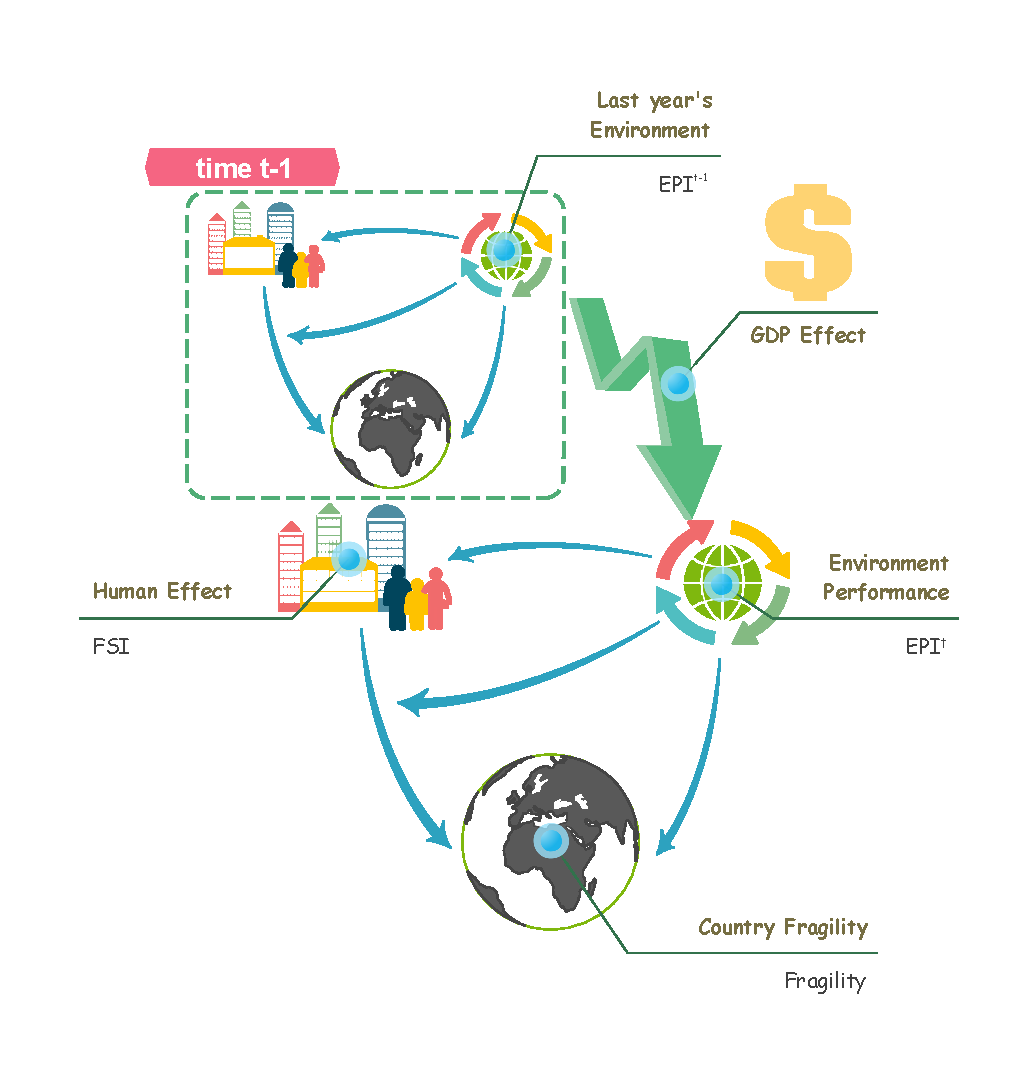
\includegraphics[width=.8\linewidth]{figs/model} 
   \caption{Hypothesis Model Illustration}
   \label{fig:model:model}
\end{figure}

\begin{figure}[t]
   \centering
   \subfigure[Moderator variable model]{
       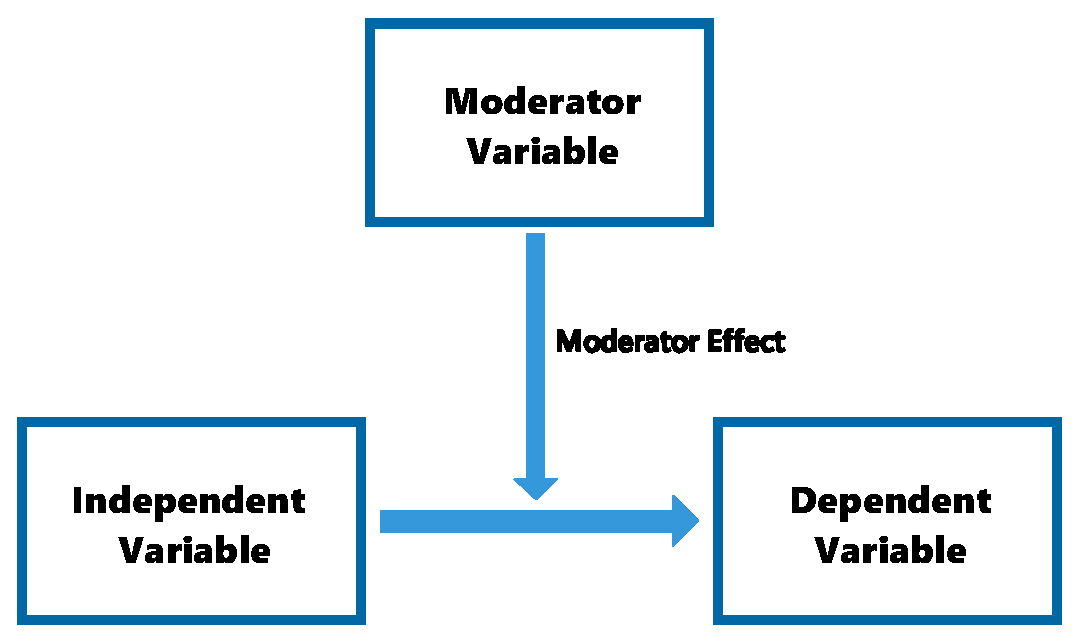
\includegraphics[width=.4\linewidth]{figs/model_moderator}
       \label{fig:model:indirect:moderator}
   } 
   \subfigure[Mediator variable model]{
       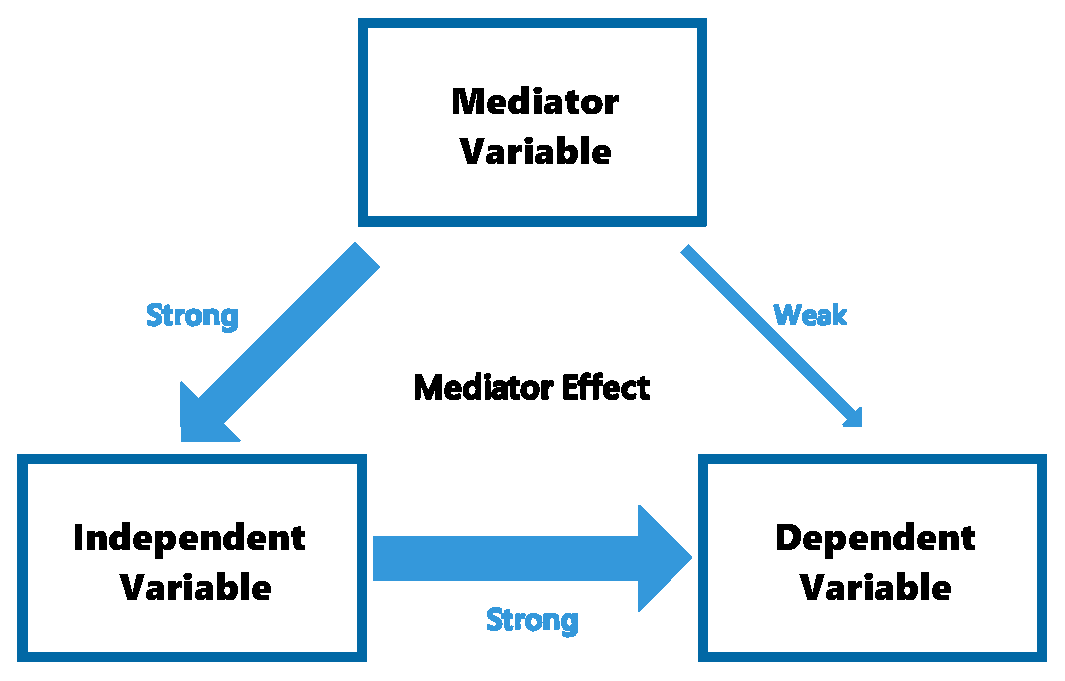
\includegraphics[width=.4\linewidth]{figs/model_mediator}
       \label{fig:model:indirect:mediator}
   }
   %\label{fig:model:indirect}
   \caption{Hypothesis models for indirect effect of environmental factors. $\EFF$ represents environmental factors, $\HFF$ represents human factors, and $\FFF$ represents state fragility. The fragility is jointly determined by $\EFF$ and $\HFF$, by two hypothesis approach.}
\end{figure}
\label{sec:model}
In this part we propose theoretical framework for our analysis of the impact of climate change on \emph{state fragility}.
\subsection{Assumptions and Model Framework}
Our hypothesis framework is illustrated in Figure~\ref{fig:model:model}.
We propose two natural assumptions, based on which we derive the basic framework of our model. 
\begin{enumerate}
   \item The \emph{state fragility}, a concept to estimate the sustainability of states, is dependent on and only on \emph{human factors} and \emph{environmental factors.} \label{model:assump:1}
   \item The environmental factors and human factors interact with each other. \label{model:assump:2}
\end{enumerate}
The assumptions are natural. Assumption~\ref{model:assump:1} requires to quantify the fragility which considers both human factors and environmental factors. We propose a novel framework to quantify fragility by incorporating the human and environmental factors into a probabilistic framework.

Assumption~\ref{model:assump:2} requires a more sophisticated analysis of the two factors, including their respective and joint effects on the fragility, and the interaction between them. We are especially interested in the effects of environmental factors, which include \emph{direct} effect, which is the influence on fragility directly imposed by environmental factors; and \emph{indirect} effect, which is the influence on fragility imposed by envirionmental factors indirectly through human factors. Two hypothesis model to explain the indirect effect is visualized in Figure~\ref{fig:model:indirect:moderator} and~\ref{fig:model:indirect:mediator}.

The direct effect of environmental factors is measured by the effect of environmental factors on fragility score, with an unbiased estimation of the effect obtained by propensity score matching~\reminder{citation}. The indirect effect of environmental factors can be explained by two hypothesis models: the \emph{moderator variable} model, as shown in Figure~\ref{fig:model:indirect:moderator}; and the \emph{mediator variable} model, as shown in Figure~\ref{fig:model:indirect:mediator}. We verify these two hypothesis.

In the following of this section, we are dedicated to enrich our model by developing several key ingredients: 
\begin{enumerate}
   \item A novel fragility score measure incorporating both environmental and human factors;
   \item The interaction pattern between human factors, envirionmental factors, and the fragility;
   \item The temporal model of a state's environmental status.
\end{enumerate}

The basic framework is sufficient to cover most of the requirements of the tasks.
Furthermore, we discuss strengthes and weaknesses respectively in each part.

\subsection{Representing the Two Factors}
\label{sec:model:rep}
\begin{table}[htbp]
   \centering
   \begin{tabular}{|c|c|} \hline 
      Notation & Description \\ \hline
      $\HFF $  & random variable of human factors \\ \hline
      $\EFF $ & random variable of environmental factors \\ \hline
      $ \FFF $ & binary random variable of fragility \\ \hline
      $\FFS $ & fragility score \\ \hline
   \end{tabular}
\end{table}

\begin{figure}[t]
    \centering
    \subfigure[FSI]{
        \includegraphics[width=.4\linewidth]{figs/epi}
        \label{fig:model:indexes:fsi}
    }
    \subfigure[EPI]{
        \includegraphics[width=.4\linewidth]{figs/epi}
        \label{fig:model:indexes:epi}
    }
    \caption{The two fragility indexes.}
    \label{fig:model:indexes}
\end{figure}

\vpara{Environmental Performance Index.} It is an index to evaluate a state's environmental performance by~\reminder{Who and citation}. It is composed of indicators in ecosystem vitality and environmental health. 

\subsection{Probabilistic Fragility Measure}
\label{sec:model:frag}
\reminder{Need to emphasize that it is logistic regression.}
In this part, we derive a novel fragile score, $\FFS$, which incorporates both environmental and human factors. The score $\FFS$ is based on probabilistic intuitions, and is therefore called the \emph{probabilistic fragility score}, or the fragility score for convenience.

Without loss of generality, we refer to regions, sovereign states, and other concerned geographical entities as states.

We assume that a state either fragile or stable, described by a binary random variable $\FFF$, where $\FFF=1$ if the considered state fragile, and $\FFF=0$ if it is stable. $\HFF$ and $\EFF$ are random variables describing the human and environmental factors of the state. For convenience, we further assume that $\EFF$ is binary, i.e. $\EFF=1$ when the state's environment is sustainable, and $\EFF=0$ when it is not. 

Consider the probability of a state being fragile, given its human and environmental factors:
\begin{equation}
    \prob{(\FFF=1|\EFF=e, \HFF)} \ \ (e=0,1)
\label{eqn:model:frag_prob}
\end{equation}

The probability given in~\ref{eqn:model:frag_prob} quantifies the extent of fragility of the state, given certain environmental and human factors. It is higher when the state is more vulnerable. However, the conditional distribution is hard to estimate. We then factorize it into a more easily calculated form: 
\begin{equation}
    \prob(\FFF=1|\EFF=e,\HFF)= \frac{\prob(\EFF=e, \FFF=1 | \HFF)}{\prob(\EFF=e | \HFF)} = \frac{\prob(\mathbf{Z}=1|\HFF)}{\prob(\EFF=e|\HFF)}\ \ (e = 0,1)
    \label{eqn:model:frag_prob_fact}
\end{equation}
In which we defined a new random variable $\mathbf{Z}=1$ if $\EFF=e,\FFF=1$ and $\mathbf{Z}=0$ otherwise.
Eqn.~\ref{eqn:model:frag_prob_fact} allows us to only estimate the conditional probability of two binary random variables given human factors $\HFF$.

For convenience of calculation, we assume linear relationships: 
\begin{eqnarray}
   \log\frac{\prob(\mathbf{Z}=1|\HFF)}{\prob(\mathbf{Z}=0|\HFF)} & = & \mathbf{W}_1\HFF + \mathbf{e}_1 \nonumber \\
   \log\frac{\prob(\mathbf{\EFF}=e|\HFF)}{\prob(\mathbf{\EFF}=1-e|\HFF)} & = & \mathbf{W}_2\HFF + \mathbf{e}_2 
   \label{eqn:model:logistic_form}
\end{eqnarray}

Where $\mathbf{W}_i$ are parameters, $\mathbf{e}_i$ are Gaussian errors, $i=1,2$.

Using the linear assumption and the logistic form in Eqn~\ref{eqn:model:logistic_form}, we obtain the estimate of the probabilities respectively:

\begin{eqnarray}
   \hat{p}_z & = & \frac{\exp(\mathbf{W}_1\HFF)}{1+\exp(\mathbf{W}_1\HFF)} \nonumber \\
   \hat{p}_e & = & \frac{\exp(\mathbf{W}_2\HFF)}{1+\exp(\mathbf{W}_2\HFF)}
   \label{eqn:model:prob_estimate}
\end{eqnarray}

In order to make the estimated probability distribution resemble the true distribution, we estimate parameters $\mathbf{W}_1, \mathbf{W}_2$ by minimizing the cross entropy loss, which is equivalent to minimizing the KL divergence~\reminder{reference needed} between the estimated distribution and the empirical distribution. \reminder{specific form omitted.}

Finally, probabilities in Eqn.~\ref{eqn:model:frag_prob_fact} is replaced by the estimates given in Eqn.~\ref{eqn:model:prob_estimate}, yielding the \emph{probabilistic fragility score}:
\begin{equation}
  \label{eqn:model:frag_score}  
  \FFS = \frac{\hat{p}_z}{\hat{p}_e}
\end{equation}

\paragraph{Notes on the fragility score.} The fragility score, $\FFS$, is derived based on probabilistic intuitions and linear assumptions. Higher $\FFS$ indicates higher risks of being fragile. However, the score $\FFS$ can be larger than one, and is, therefore, not in form of probability. However, it does not hurt its applicability: if the estimated $\hat{p}_z$ is larger than $\hat{p}_e$, we have even more reasons to believe that the considered state is fragile. 

\subsection{Modeling the Interaction between Variables}
We then begin to model the relationship between the three variables: environmental factors $\EFF$, human factors $\HFF$, and the fragility score $\FFS$. 

\subsubsection{Direct Effect of Environmental Factors} In order to measure the effect of environmental factors on fragility score, a naive approach would be to sample states of both sustainable environment and unsustainable environment, and compare their average fragility score. Formally, write $s^0_f$ as the average fragility score of the sustainable group, and $s^1_f$ as the average fragility score of the unsustainable group. One then compares the difference $s^*_f=s^0_f - s^1_f$.

The above approach gives, however, biased estimation, because the apparent difference between these two groups may be depend on human factors that affected whether or not a state's environment is sustainable, instead of the environmental status per se. For example, the approach might compare scores of the states that are environmentally unsustainable and in political turmoil, with the scores of the states that are environmentally sustainably and politically stable. The difference of political status results in unbiased estimate of the effect of environmental factors.

To control for the differences of human factors between the sustainable group and the unsustainable group, we use the propensity score matching, a statistical technique that attempts to estimate unbiasly the effect of a variable, in this case, the environmental status.

Formally, the propensity score of a certain state is defined as the conditional probability of the environmental status given its human factors,
\begin{equation}
   p=\prob(\EFF=1|\HFF)
   \label{eqn:model:propensity}
\end{equation}
\reminder{environmental status? environmental factors? they are probably different.}
In order to estimate the probability, we adopt similar procedures used in Section~\ref{sec:model:frag}, using the score of logistic regression, $\hat{p}$, of human factors $\HFF$ against environmental status $\EFF$. Then we match each of the unsustainable states to one sustainable state on propensity score, by using \emph{Nearest Neighbor Matching}: each unsustainable state is matched to the sustainable state whose propensity score is the closest. As such, a new data set in which the sustainable group and the unsustainable group and their propensity scores are balanced, is obtained. 

Based on the newly obtained data set, we calculate the adjusted score difference:
\begin{equation}
   \hat{s}^*_f=\hat{s}^0_f - \hat{s}^1_f.
   \label{eqn:model:score_diff_adj}
\end{equation}

Where $\hat{s}^0_f$, $\hat{s}^1_f$ are average scores of the sustainable and unsustainable group, drawn from the data set obtained by PSM.

\subsubsection{Indirect Effect of Environmental Factors}
\label{sec:model:indirect}
In order to measure the indirect effect of environmental factors $\EFF$, we propose two candidate models: the moderator variable model, and the mediator variable model.

\reminder{is the difference clearly explained?}
The moderator variable model assumes that the environmental factors influence the fragility score, and the relationship is calibrated by the effect of human factors. 
In this case, the human factors $\HFF$ are called \emph{the moderator variable}, as illustrated in Figure~\ref{fig:model:indirect:moderator}.\reminder{reference.}

The mediator variable model assumes that the environmental factors and human factors jointly influence the fragility score.
Furthermore, the environmental factors influence the fragility score both directly, and indirectly through the human factors. The illustration of this model is as in Figure~\ref{fig:model:indirect:mediator}.\reminder{reference.}

\vpara{Moderator variable model.}
The model is written as 
\begin{equation}
    \FFS = \mathbf{W}_1\HFF + W_2\EFF + \sum_{i=1}^p \beta_i h_i \EFF 
    \label{eqn:model:moderator_model}
\end{equation}
where $\HFF=\left[ h_1,\ldots,h_p \right]'$, and $h_i$ is the $i$th component of $\HFF$, indicating a specific factor. $\mathbf{W}$ and $\beta_i$ are parameters.

The term, $\sum_{i=1}^p\beta_i h_i$, represents the effect of each human factor on the relation between the environmental factor and the fragility score, since by taking partial derivative, we observe that 
\begin{equation*}
    \frac{\partial s_f}{\partial \EFF} = W_2 + \sum_{i=1}^p \beta_i h_i
\end{equation*}
The derivative indicates that the effect of environmental factor $\EFF$ comes from both itself, described by $W_2$, and each human factor $h_i$, described by $\beta_i$. If the factor $h_i$ has no effect on the relation, then $\beta_i$ should be close to zero. Consider, therefore, the following statistical test:
\begin{equation}
    H_0: \beta_1=\beta_2=\ldots=\beta_p
    \label{eqn:model:moderator:testall}
\end{equation}
The rejection of $H_0$ shows that the moderator effect of $\HFF$ is significant. 
Furthermore, we wish to specifically investigate the effect of each factor. Hence in the following test,
\begin{equation}
   H_0:\beta_i=0 
   \label{eqn:model:moderator:testi}
\end{equation}
if $H_0$ is rejected, we are confidence to say that the moderator effect of $h_i$ is statistically significant.

If the moderator effect is indeed significant, then the extent of the effect of $\HFF$ is then quantified by $\mathbf{\beta} = \left[\beta_1,\ldots,\beta_p\right]'$ and respective components.

\vpara{Mediator variable model.} 
\reminder{Human factors are multivariate. Maybe consider human factors only as FSI, a single variable.}

We first declare the following values:
\begin{itemize}
   \item $b_1$: the coefficient of the linear regression model, in which $\EFF$ predicts $\FFS$.
   \item $b_2$: the coefficient of the linear regression model, in which $\HFF$ predicts $\FFS$.
   \item $b_3$: the coefficient of $\EFF$ in the linear regression model in which $\EFF$ and $\HFF$ jointly predicts $\FFS$.
   \item $b_4$: the coefficient of $\HFF$ in the linear regression model in which $\EFF$ and $\HFF$ jointly predicts $\FFS$.
\end{itemize}

First, we need to verify by statistical tests that $b_1$ and $b_2$ are significantly nonzero.

If $\HFF$ indeed acts as a mediator variable, by model assumption, $b_4$ is significantly nonzero. Furthermore, since $\EFF$ indirectly influences $\FFS$ through $\HFF$, the explaining power of $\EFF$ alone should be reduced once $\HFF$ is introduced. In this case, $b_3 < b_1$.

If all the above four conditions hold significantly, we are confident to say that human factors act as mediator variables, through which the environmental factors influence the fragility score.

\subsection{Temporal Model}
% In Section~\ref{sec:model1} we analyzed in depth the relationship between the three variables: the environmental factors $\EFF$, the human factors $\HFF$, and the fragility score $\FFF$. 
In order to better model climate change, we further consider time as a variable, and investigate how climate change would have influenced the fragility of states. Specifically, we choose China as an example state, and illustrate how and when it would reach a tipping point 
\section{Experiments}
\label{sec:exp}
\subsection{Data Preparation}
\label{sec:exp:prep}

\vpara{Dataset.}
% years

We prepared several representative datasets for the variables we need: $\EFF$, $\HFF$, and $\FFF$.
\vpara{Fragility Score Index.}

\vpara{Environmental Performance Index.}

\vpara{Other Indicators.}

\subsection{Calculation of Fragility Score}
In order to calculate fragility score defined in Section~\ref{sec:model:frag}, we need to identify, a priori, which states are fragile and which states are environmentally unstable. 
In order to achieve so, we determine that a state is fragile, i.e. $\FFF=1$, if its FSI score is higher than a certain threshold $F_0$, and a state is environmentally fragile, i.e. $\EFF=1$, if its EPI score is lower than a certain threshold $E_0$. 
The thresholds are chosen differently for each year, because the indexes of different years aren't necessarily calculated using the same methodology.
Therefore, thresholds for each year are chosen to guarantee that the fragile states and environmentally fragile states occupy approximately $30\%$ of the states, respectively. As such, each state's status of fragility and environmental fragility is approximated by HSI and EPI indexes. Furthermore, we use the 12 indicators used in the calculation of FSI, specified in \reminder{specify somewhere}, as components of human factors $\HFF = \left[ h_1\ldots h_12 \right]$.

Hence, all variables needed for the calculation of our fragility score, including $\HFF, \EFF, \FFF$, are specified for each state. Logistic regression was run as described in Section~\ref{sec:model:frag} to obtain fragility score of each state. Finally, we visualize the relationship between the score and the two indexes in Figure~\ref{fig:exp:frag_relation}.
\begin{figure}[htbp]
    \centering
   \subfigure[EPI]{
       \includegraphics[width=.4\textwidth]{figs/epifs}
       \label{fig:exp:frag_relation:epi}
   }
   \subfigure[FSI]{
       \includegraphics[width=.4\textwidth]{figs/fsifs}
       \label{fig:exp:frag_relation:fsi}
   }
   \caption{Relationship between Fragility Score $\FFS$ and FSI and EPI.} 
   \label{fig:exp:frag_relation}
\end{figure}
Figure~\ref{fig:exp:frag_relation:epi} shows that states with lower EPI indexes have higher scores in general, but the variance is high when the environment is worsened. Figure~\ref{fig:exp:frag_relation:fsi} shows that states with higher FSI obtain higher scores. 
The figures show that HSI majorly determines $\FFS$, while EPI acts as an adjustment.

\vpara{Consistency Test.}
In order to show that $\FFS$ is a reasonable criterion of states' fragility, we need to make sure that a state which is completely better than another state, i.e. with higher EPI and lower FSI, obtains lower $\FFS$. In this case, we call that the two states are \emph{inconsistent}.
We therefore define the average reverse number order $r$: 
\begin{equation}
   r\triangleq \frac{1}{2N}\sum_{k=1}^N \frac{r_k}{N}  = \frac{1}{2N^2}\sum_{k=1}^N r_k
   \label{eqn:exp:reverse_order}
\end{equation}
where for the $k$th state in the dataset, $r_k$ is the number of other states that inconsistent with it.

The $r_k$ calculated for the indexes in the year of 2017 is $0.01764$, which is sufficiently low to bring confidence to the fragility score $s_f$.

\begin{figure}[htbp]
    \centering
    \subfigure[General Effect] {
        \includegraphics[width=.48\linewidth]{figs/fragility_treat}
        \label{fig:exp:direct:general}
    }
    \subfigure[Specific Countries] {
        \includegraphics[width=.48\linewidth]{figs/compare_score}
        \label{fig:exp:direct:specific}
    }
    \caption{Direct Effect of Environmental Factors.}
\end{figure}

\subsection{Indirect Effect of Environmental Factors}

To measure the indirect effect of environmental factors, we modeled several regression models in Section~\ref{sec:model:indirect}. Specifically, we choose the EPI index and FSI index described in Section~\ref{sec:exp:prep} to represent the environmental factors $\EFF$ and human factors $\HFF$, respectively. The indexes are scaled and centralized, such that a comparsion of coefficients is meaningful.
\begin{table}[htbp]
    \centering
   \begin{tabular}{|l|ccc|} \hline
      Variable & $\EFF$ & $\HFF$ & $\EFF\times\HFF$ \\ \hline
      Coefficient & 0.17 & 0.91 & 0.06 \\ \hline
      P-value & 0.31 & 0.00 & 0.69679 \\ \hline
      Significant & No & Yes & No  \\ \hline
   \end{tabular} 
   \caption{Moderator variable model of human factors.}
   \label{tab:exp:moderator}
\end{table}

\vpara{Moderator Effect.}
The regression parameters and their p-value is listed in Table~\ref{tab:exp:moderator}. Lower p-value indicates that the original hypothesis that was tested is insignificant. We determine that if the p-value lower a certain threshold, $0.05$, we would reject the hypothesis. Since our hypothesis detailed in Section~\ref{sec:model:indirect} is that the coefficient is zero, p-value lower than $0.05$ would show that the effect of the corresponding variable is significant.

Table~\ref{tab:exp:moderator} shows that the moderator effect is not significant; therefore we would reject the hypothesis that the human factors act as a moderator of the relation between the environmental factors and the fragility.

\begin{table}[htbp]
    \centering
    \begin{tabular}{|l|cccc|} \hline
        Variable & Model & Coef. & p-val. & Sign.  \\ \hline
        % \multirow{2}{*}{Human factors} & $\FFF\sim\HFF$ & -0.8349 & $<2e-16$ & Yes \\ \cline{2-5}
        Human factors & $\FFF\sim\HFF + \EFF$ & 1.009 & $<2e-16$ & Yes  \\ \hline        
        \multirow{3}{*}{Environmental factors} & $\HFF\sim\EFF$ & -0.8349 & $<2e-16$ & Yes \\ \cline{2-5}
        & $\FFF\sim\EFF$ & -0.6152 & $<2e-16$ & Yes \\ \cline{2-5}
        & $\FFF\sim\HFF+\EFF$ & 0.2272 & 0.00773 & Yes \\ \hline        
    \end{tabular}
    \caption{Mediator variable effect of human factors. The column Model tells the regression model, in which the left hand of $\sim$ is the dependent variable, and the right hand are the independent variables used in the regression model.}
    \label{tab:exp:mediator:general}
\end{table}
    
\vpara{Mediator Effect.}
Table~\ref{tab:exp:mediator:general} shows the result of the test of the mediator effect of human factors, represented by the FSI index. The results show that the effect of human factors on fragility is significant, and that the effect of environmental factors on fragility is significant, by corresponding coefficients in models $\FFF\sim\HFF+\EFF$ and $\HFF\sim\EFF$. In both models of $\FFF\sim\EFF$ and $\FFF\sim\HFF+\EFF$, the effects of human factors on the fragility are significant; furthermore, the absolute value of the coefficient is reduced by approximately $0.4$ once $\HFF$ is introduced. Therefore, the human factors act as a mediator variable, through which the environmental factors influence fragility. Furthermore, model $\FFF\sim\EFF$ shows that environmental factors also influence fragility directly. As such, a statistical proof of the mediator variable model in Section~\ref{sec:model:indirect} is complete.

We are also interested in how the influence of environmental factors propagate through human factors. Therefore, we choose the 12 indicators used in the calculation of HSI index~\reminder{citation}, and construct a new regression model: $\FFF\sim\EFF+h_1+\ldots+h_12$, where $h_i$ is an individual factor. However, not all of the indicators are significant, therefore we attempt to find best subset of indicators that are significant by stepwise regression: at each step, we remove from the regression model an indicator that is statistically insignificant. Since previously removed indicator could be significant in the new model, we add at each step a previously removed indicator that has become significant to the regression model, if there is one. We stop when there is no insignificant indicator to remove and no significant indicator to add. 

The used subset of indicators, their coefficients and significance are shown in Table~\ref{tab:exp:mediator:subset}.
Experiments show that the impact of environmental change propagates mainly through demographic pressures, human flight and brain drain, and human rights. It also flows through group grievance in a less significant manner. Furthermore, it goes through Economy and refugee flows slightly. 

\begin{table}[htbp]
   \centering 
   \begin{tabular}{|l|ccc|} \hline
      Variable & Coef. & p-value & Sign. \\ \hline 
       DP & 0.3009 & 0.00691 & High \\ \hline
       HFBD & 0.2579 & 0.00287 & High \\ \hline
       HR & 0.2424 & 0.00196 & High \\ \hline
       GG & 0.1643 & 0.01824 & Medium \\ \hline
       Econ. & 0.1380 & 0.08155 & Low \\ \hline
       RI & 0.1275 & 0.08768 & Low \\ \hline
   \end{tabular}
   \caption{Best subset of mediator indicators. Rows are respectively: Demographic Pressures, Human Flight and Brain Drain, Human Rights, Group Grievance, Economy, and Refugees and IDPs.}
   \label{tab:exp:mediator:subset}
\end{table}

\vpara{Conclusion on Indirect Effects.} Above experiments show that:
\begin{itemize}
   \item The environmental factors and human factors both directly influence fragility;
   \item Environmental factors also influence human factors, and human factors act as a mediator variable to pass the influence of the environmental factors to fragility 
\end{itemize}
Which is illustrated in Figure~\ref{fig:model:indirect:mediator}. 

\subsection{Temporal Model}
\label{sec:exp:temporal}


\subsection{Regional Model}
\label{sec:exp:regional}
\input{related.tex}
\section{Conclusion}
\label{sec:conclusion}

We proposed a novel probabilistic framework to evaluate a state's fragility. Based on this, we analyzed the direct and indirect of environmental factors on fragility, and the interaction between environmental and human factors in their joint contribution to fragility. 

We also proposed a temporal framework to forecase future environmental change. Our model found that moderate economic growth balances the trade-off between fast economic development and environmental damage in the long term.

\balance
\bibliographystyle{acm}
\bibliography{mybibtex}

\end{document}
